\documentclass{beamer}
\usepackage{relsize}
\usepackage{color}

\usepackage{listings}
\usetheme{CambridgeUS}
%\usepackage{beamerthemesplit} % new
\usepackage{enumitem}
\usepackage{amsmath}                    % See geometry.pdf to learn the layout options.
\usepackage{amsthm}                   % See geometry.pdf to learn the layout options. There
\usepackage{amssymb}                    % See geometry.pdf to learn the layout options.
\usepackage[utf8]{inputenc}
\usepackage{graphicx}
\usepackage[english,bulgarian]{babel}

\usepackage{caption}
\usepackage{tikz}

\usetheme{CambridgeUS}
\usecolortheme{crane}

\lstset{language=C++,
                basicstyle=\ttfamily,
                keywordstyle=\color{blue}\ttfamily,
                stringstyle=\color{red}\ttfamily,
                commentstyle=\color{green}\ttfamily,
                morecomment=[l][\color{magenta}]{\#}
}

\newtheorem{mydef}{Дефиниция}[section]
\newtheorem{lem}{Лема}[section]
\newtheorem{thm}{Твърдение}[section]

\DeclareMathOperator{\restrict}{\upharpoonright}

\setitemize{label=\usebeamerfont*{itemize item}%
  \usebeamercolor[fg]{itemize item}
  \usebeamertemplate{itemize item}}

\setbeamercovered{transparent}

\captionsetup{font=tiny} 

\begin{document}
\title[Сериализация и десериализация]{Сериализация и десериализация}
\frame{\titlepage}

\section{Сериализация и десериализация}
\subsection{}


\begin{frame}[fragile]
  \frametitle{Сериализация}
  \begin{tikzpicture}[remember picture,overlay]
    \node[xshift=0,yshift=-14mm,anchor=north] at (current page.north){%
    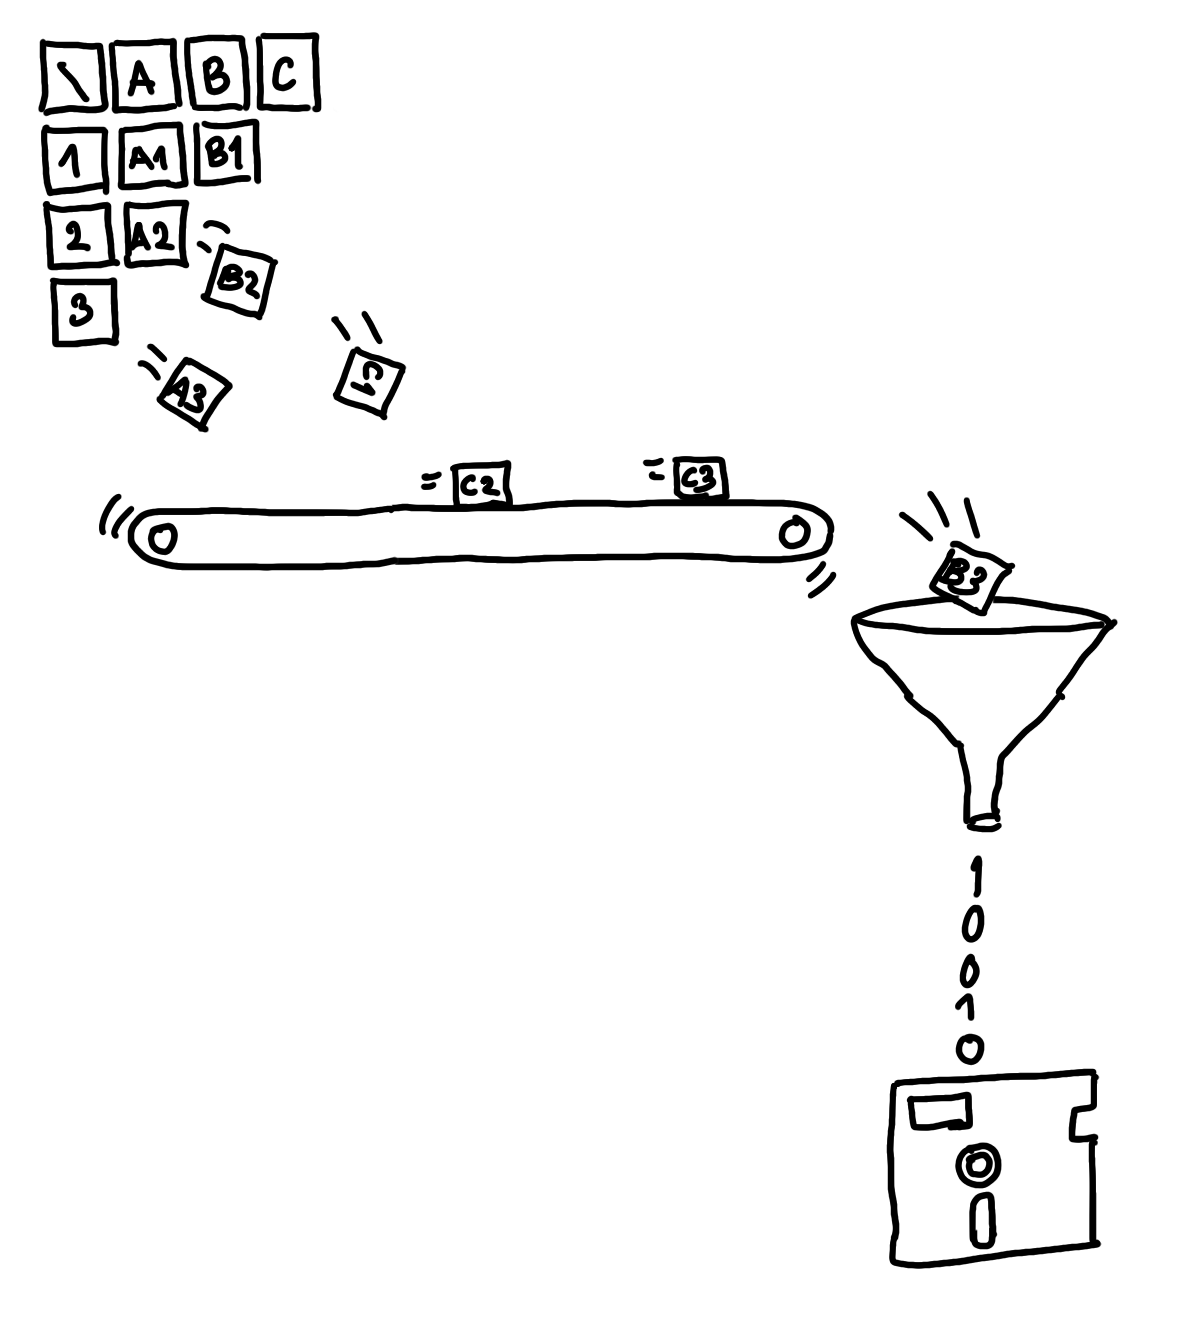
\includegraphics[width=70mm]{images/serialization}};
  \end{tikzpicture}
\end{frame}


\begin{frame}[fragile]
  \frametitle{Сериализация}

\begin{lstlisting}[basicstyle=\small,language=Haskell]
data Gender = M | F
    deriving (Show,Eq)
data Person = Person {name :: String, 
                      gender:: Gender, 
                      birthdate :: (Int,Int,Int)}
    deriving (Show,Eq)
people :: [Person] = 
    [Person {name = "Kalin Georgiev", 
             gender = M, 
             birthdate = (01,01,1981)},
     ...]
\end{lstlisting}

\end{frame}


\begin{frame}[fragile]
  \frametitle{show и read}

\begin{itemize}
  \item Сериализация и десериализация с \verb#show# и \verb#read#
  \item Запис на текст във файл
\end{itemize}

\bigskip

\begin{lstlisting}[basicstyle=\small,language=Haskell]
writeFile "test.txt" $ show people
\end{lstlisting}

\end{frame}


\begin{frame}[fragile]
  \frametitle{CSV}

Форматът Comma Seprated Values, \verb#CSV#

\begin{verbatim}
name,gender,birthdate
Kalin Georgiev,M,01-01-1981
Maria Ivanova,F,05-05-2003
\end{verbatim}

\begin{lstlisting}[basicstyle=\small,language=Haskell]
writeFile "data.csv" $ 
          concat $ map ((++"\n").writePerson) people
\end{lstlisting}


\end{frame}


\begin{frame}[fragile]
  \frametitle{Десериализация}
  \begin{tikzpicture}[remember picture,overlay]
    \node[xshift=0,yshift=-14mm,anchor=north] at (current page.north){%
    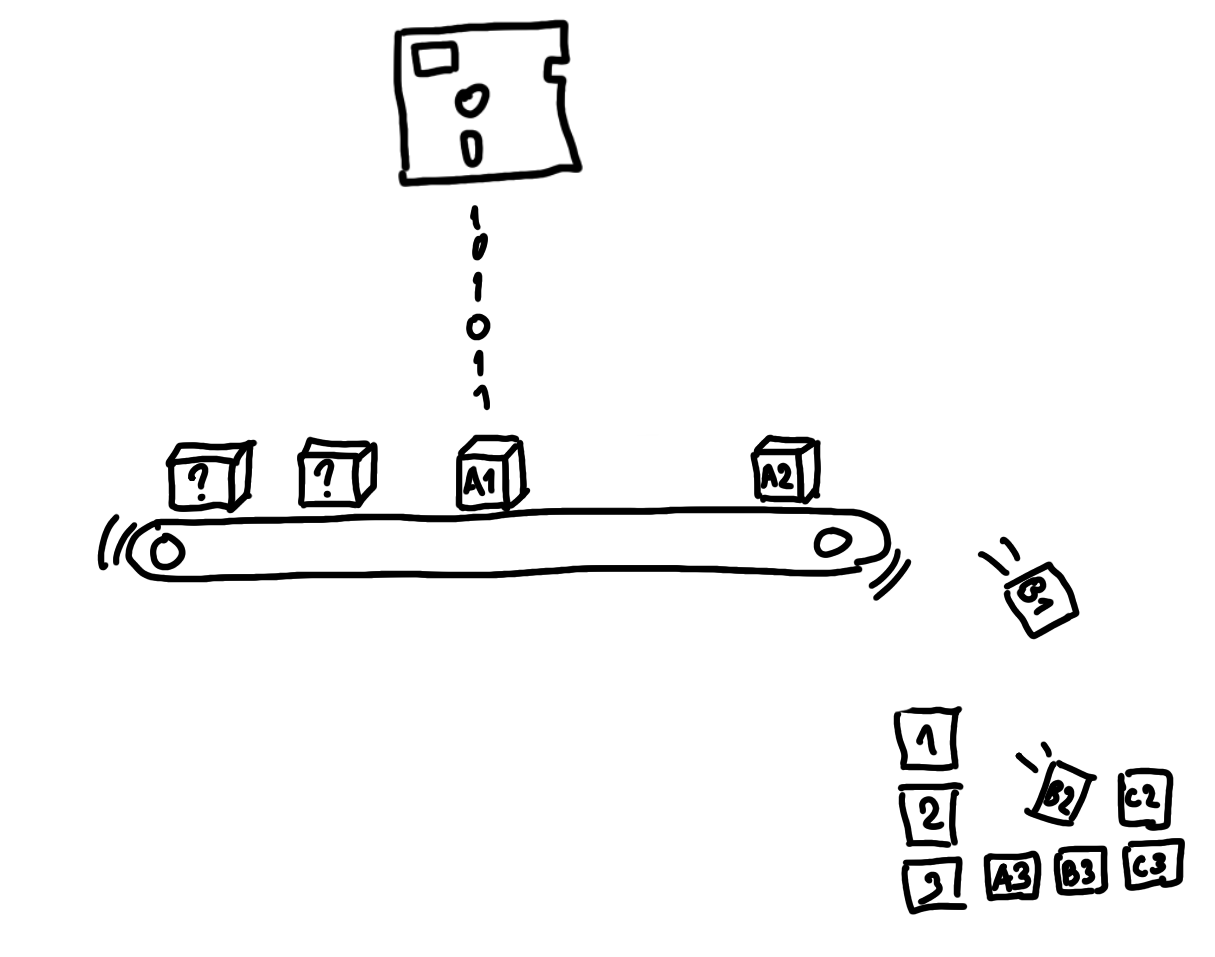
\includegraphics[width=80mm]{images/deserialization}};
  \end{tikzpicture}
\end{frame}


\begin{frame}[fragile]
  \frametitle{Четене от файл}


\begin{lstlisting}[basicstyle=\small,language=Haskell]
readPeople :: IO ([Person])
readPeople = do
    contents <- readFile "data.csv"
    return $ map readPerson $ lines contents  
\end{lstlisting}

\bigskip

\begin{itemize}
  \item \verb#readFile# извършва мързеливо четене
\end{itemize}


\end{frame}

\begin{frame}[fragile]
    \frametitle{}
  
  \centerline{Благодаря за вниманието!}
\newcommand{\license}[1]{
  \begin{tikzpicture}[remember picture,overlay]
      \node[xshift=0mm,yshift=13mm,anchor=south east] at (current page.south east)
      {\tiny{Материалите са разработени от Калин Георгиев за курсовете по програмиране на ФМИ, СУ}};
      \node[xshift=0mm,yshift=10mm,anchor=south east] at (current page.south east)
      {\tiny{Creative Commons Attribution-NonCommercial-ShareAlike 4.0 International}};
      \node[xshift=0mm,yshift=5mm,anchor=south east] at (current page.south east){%
      \includegraphics[width=30mm]{{#1}/license}};
    \end{tikzpicture}
}
\license{../../..}
 
\end{frame}  

\end{document}


\begin{columns}[t]
  \begin{column}{0.2\textwidth}

\relscale{0.63}
\begin{lstlisting}
\end{lstlisting}
\relscale{1}

  \end{column}
  \begin{column}{0.8\textwidth}

  \end{column}
\end{columns}


